%% IJCAI-format draft. Upload the official IJCAI author-kit files (ijcai27.sty or ijcai26.sty, named.bst)
%% next to this file in Overleaf. Without them the file still compiles with a close two-column fallback.
\IfFileExists{ijcai27.sty}{\def\ijcaistyle{ijcai27}}{\IfFileExists{ijcai26.sty}{\def\ijcaistyle{ijcai26}}{}}
\ifdefined\ijcaistyle
  \documentclass{article}
\else
  \documentclass[twocolumn,10pt]{article}
\fi
\pdfpagewidth=8.5in
\pdfpageheight=11in
\ifdefined\ijcaistyle
  \usepackage{\ijcaistyle}
\else
  \usepackage[letterpaper,margin=0.75in,columnsep=0.25in]{geometry}
  \usepackage[round]{natbib}
\fi
\usepackage{times}
\usepackage{soul}
\usepackage{url}
\usepackage[utf8]{inputenc}
\usepackage[small]{caption}
\usepackage{graphicx}
\usepackage{amsmath}
\usepackage{amssymb}
\usepackage{amsthm}
\usepackage{booktabs}
\usepackage{xcolor}
\urlstyle{same}

\newcommand{\todo}[1]{\textcolor{red}{[TODO: #1]}}
\newcommand{\pilot}{\textsuperscript{\textcolor{gray}{$\dagger$}}}
\newcommand{\sg}{\operatorname{sg}}
\newcommand{\JS}{\operatorname{JS}}

\title{Policy Similarity Is Not Team Membership:\\ Diagnosing Selective Critic Sharing among Latent Teams}
\author{Anonymous submission}

\begin{document}
\maketitle

\begin{abstract}
Selective sharing between learning agents is attractive when agents belong to latent teams with different
objectives: sharing with teammates may accelerate learning, while sharing with non-teammates may be useless
or harmful. A natural decentralised recipe is to infer whom to share with from behavioural similarity.
We study this recipe in a two-team warehouse task with hidden team membership, team-relative observations and
individual rewards, using a policy-similarity-gated critic distillation method (PGCT) that compares agents'
action distributions on a fixed bank of canonical probe observations. Frozen-policy diagnostics show that
probe-based policy similarity does not identify teammates (same-team AUROC 0.375--0.500 across six
checkpoints), whereas task events that an agent witnesses in its own field of view identify every teammate
within one episode. Training from scratch with one seed (a pilot, not a statistical result), the gate admits
most pairs early on but, after about 2M steps, links almost exclusively agents of different teams; the agents
it links are those with similar roles and skill rather than those with the same objective. Critic sharing
with ground-truth teammates nevertheless gave the earliest and highest learning curve in this pilot, and
the number of agents that learned to deliver at all increased with the breadth of sharing. Re-running
the same seed showed that sharing variants are not bit-reproducible and that their onsets can shift by
two million steps. We conclude that behavioural similarity confounds team, role and skill, and we outline
the evidence needed before claiming that inferred teams improve learning.
\end{abstract}

\section{Introduction}
In many multi-agent systems the agents that share an environment do not share an objective. Warehouse robots
of different clients, vehicles of different fleets, or players of different teams act in the same space, observe
each other locally, and learn simultaneously. Sharing learned knowledge---parameters, experience or value
estimates---is a well-established way to improve sample efficiency in multi-agent reinforcement learning
(MARL)~\cite{christianos2020seac,christianos2021seps}, but it presupposes that the agents involved are compatible.
When team membership is latent, an agent must first decide \emph{with whom} to share.

A tempting decentralised answer is to share with agents that \emph{behave} similarly. This is the idea behind
the method we analyse, policy-gated critic transfer (PGCT): agents compare their action distributions on a fixed
bank of probe observations, and an agent distils the critic of a neighbour whose policy is close enough.
The idea rests on a chain of assumptions: (i) teammates behave more similarly than non-teammates, (ii) the
probe bank exposes that difference, and (iii) teammates' value functions are more compatible, so their critics
are useful targets. Each link can fail. Teammates may take different roles; non-teammates may solve
symmetric sub-problems in the same way; and with individual rewards, teammates compete for the same requests.

This paper is a diagnostic study of that chain in a controlled environment. We separate three questions:
\begin{itemize}
  \item \textbf{RQ1 (identifiability).} Does the information available to an agent identify its teammates, and
    does probe-based policy similarity carry that information?
  \item \textbf{RQ2 (value of the right partners).} When agents learn from scratch, does sharing critics with the
    ground-truth team help compared with no sharing and with sharing with everyone?
  \item \textbf{RQ3 (what the gate does).} Which partners does a similarity gate actually select during training,
    and why?
\end{itemize}

Our contributions are: (1) a problem formulation and evaluation protocol that keep team identifiability, oracle
sharing value and the behaviour of an inferred gate apart, with the realised donor allocation logged at every
update; (2) evidence that, in a team-symmetric warehouse task, probe-based policy similarity does not identify
teams while locally witnessed task events do; (3) a from-scratch pilot in which the similarity gate drifts to
cross-team links between agents with similar roles, while oracle-team sharing gives the best learning curve and
broader sharing lets more agents learn; and (4) a reproducibility analysis showing that sharing variants are not
bit-reproducible even with identical seeds and initial weights. We state clearly which results are single-seed
pilots and what is still missing (multiple seeds, a goal-separated environment variant, and an online
team-inference method).

\section{Related Work}
\textbf{Sharing in MARL.} Parameter sharing is standard in cooperative MARL. Selective parameter sharing (SePS)
clusters agents by a learned encoding of their transitions and shares parameters within clusters
\cite{christianos2021seps}; heterogeneity-aware methods decide dynamically which agents share
\cite{hu2025heterogeneity}. Shared experience actor-critic (SEAC) lets agents learn from each other's experience
with importance weighting \cite{christianos2020seac}. These works mainly target cooperative settings where all
agents optimise a common objective; we study the case where membership in an objective group is hidden and
only critic predictions are shared, while actors remain independent.

\textbf{Decentralised critics.} Networked actor-critic methods reach consensus on critic parameters over a
communication graph with convergence guarantees for linear approximation \cite{zhang2018networked}. In our setting
the communication graph (physical proximity) and the team structure differ, rewards are individual, and the
critics are recurrent networks aligned only on probe inputs through a distillation loss \cite{rusu2016policy}.

\textbf{Roles and independent learning.} Role-based methods such as RODE discover roles from action effects
\cite{wang2021rode}. Roles and teams are different latent variables: teammates may have different roles and
non-teammates the same role, which is exactly the confound we observe. Our learners are independent recurrent PPO
agents \cite{schulman2017ppo,dewitt2020ippo}; MAPPO \cite{yu2022mappo} uses a centralised critic and is a natural
baseline for a later stage of this work. We report evaluation protocols in line with the recommendations of
\cite{agarwal2021precipice}.

\section{Problem Setting}
We consider a partially observable stochastic game with agents $i\in\{1,\dots,N\}$, local observation histories
$h_i^t$, actions $a_i^t$ and individual rewards $r_i^t$. Each agent belongs to a latent team $z_i\in\{1,\dots,K\}$
that determines its objective (which requests it serves and where it delivers). An agent knows its own objective
through team-relative observation channels but does not observe $z_j$ of other agents. Agents within
communication range form a time-varying neighbourhood $\mathcal{N}_i(t)$ and may exchange model outputs on a
common, pre-agreed probe bank; they do not exchange raw observations or team labels.

\textbf{Environment.} We use a two-team variant of the multi-robot warehouse \cite{papoudakis2021benchmarking} on an
$11\times10$ map (\emph{E1}) with four agents (agents 1 and 3 form team red, agents 2 and 4 team blue). Each team
always has two outstanding shelf requests and its own delivery goal; the two goals are adjacent at the bottom
centre. Half of each team's shelves are placed in the other team's half of the map. Observations are egocentric
$11\times11$ semantic grids plus ego features; channels such as ``requested shelf'' and ``relevant goal'' are
defined relative to the observer's team. Rewards are individual: an agent is rewarded for its own deliveries
and returns of its team's requested shelves, plus small shaping terms. Under team-relative observations and
adjacent goals the two teams face the same decision problem; E1 is therefore a \emph{team-symmetric} condition in
which team identity should matter little for value prediction. We also define \emph{E1-F}, identical except that
the team goals are moved to opposite bottom corners, so that the teams' correct behaviour diverges when no goal is
in view.

\section{Methods Compared}
All methods use independent recurrent PPO actors and critics (GRU, 128 units) trained from random initialisation;
for a given seed all methods start from bit-identical weights. They differ only in an auxiliary critic
distillation term. Let $\mathcal{Q}=\{q_m\}_{m=1}^{M}$ be a fixed bank of probe observations ($M=48$, generated
deterministically from the environment layout, sequence length one, zero initial hidden state).
For receiver $i$ with donor weights $\alpha_{ij}$,
\begin{equation}
  \mathcal{L}_i = \mathcal{L}^{\mathrm{PPO}}_i + \lambda_{\mathrm{peer}} \sum_{j\in\mathcal{N}_i(t)} \alpha_{ij}\,
  \frac{1}{M}\sum_{m=1}^{M}\big(V_i(q_m) - \sg[V_j(q_m)]\big)^2 ,
\end{equation}
with $\lambda_{\mathrm{peer}}=0.01$ and $\sg$ the stop-gradient. The methods differ in the gate $g_{ij}\in\{0,1\}$,
and $\alpha_{ij}=g_{ij}/\sum_k g_{ik}$ over current neighbours.
\begin{itemize}
  \item \textbf{IPPO}: no distillation ($g_{ij}=0$).
  \item \textbf{Oracle-team}: $g_{ij}=\mathbf{1}[z_i=z_j]$ (privileged reference, not an upper bound).
  \item \textbf{All-peer}: $g_{ij}=1$ for every neighbour.
  \item \textbf{PGCT}: every five updates, neighbours compare their policies on the probe bank,
  \begin{equation}
    D_{ij} = \frac{1}{M}\sum_{m=1}^{M} \JS\big(\pi_i(\cdot\mid q_m),\, \pi_j(\cdot\mid q_m)\big),
  \end{equation}
  maintain an exponential moving average $\bar D_{ij}\leftarrow(1-\beta)\bar D_{ij}+\beta D_{ij}$ ($\beta=0.35$),
  and open the gate $g_{ij}=\mathbf{1}[\bar D_{ij}<\tau]$ ($\tau=0.12$) after a 100-update warm-up and at least eight
  measurements.
\end{itemize}
We log the realised allocation $\alpha$ at every update, so ``transfer'' below always refers to distillation that
actually took place, not to gate candidates.

\section{RQ1: Is Team Membership Identifiable?}
\label{sec:rq1}
\textbf{Protocol.} We froze six checkpoints from earlier curriculum and continuation runs (E1 and a larger map E2;
one training seed) and ran each policy for 20 episodes of 500 steps. For every agent pair we computed:
probe-JS on the canonical bank; history-JS between the two policies on the agents' own observation histories;
the JS divergence between visited-cell distributions; and \emph{local task evidence}: pickups and deliveries by
another agent that fall inside the observer's own $11\times11$ window, classified with the observer's own
team-relative channels (``is this shelf requested for my team?'', ``is this goal mine?''). We verified on 2{,}146
events that every counted event was visible and correctly labelled in the observer's actual observation.
Team labels are used only for scoring.

\begin{table}[t]
\centering
\small
\resizebox{\columnwidth}{!}{%
\begin{tabular}{lcccc}
\toprule
Model & Probe-JS & History-JS & Occupancy & Local evidence \\
\midrule
Stage03 (E1) & .500 & .282 & .379 & 1.000 \\
E1 IPPO & .375 & .267 & .408 & 1.000 \\
E1 PGCT & .375 & .267 & .333 & 1.000 \\
E2 IPPO & .375 & .810 & .867 & 1.000 \\
E2 PGCT & .500 & .853 & .821 & 1.000 \\
Stage04 PGCT & .500 & .291 & .365 & 1.000 \\
\bottomrule
\end{tabular}}
\caption{Same-team AUROC of pairwise scores (1 = teammates always score higher; 0.5 = chance). Frozen
checkpoints of one training seed, 20$\times$500 steps each.}
\label{tab:identifiability}
\end{table}

\textbf{Results.} Table~\ref{tab:identifiability} shows that local task evidence separates teammates perfectly
in every checkpoint, and identified every teammate within the first episode. Probe-JS is at or below chance
(0.375--0.500), and history-JS is \emph{below} chance on the E1 checkpoints (0.27--0.29): teammates behave
\emph{less} alike than non-teammates. On a larger map (E2) history and occupancy carry team information
(0.81--0.87), but the probe bank does not.

Two properties of the canonical bank explain part of this. Only 26 of its 48 inputs are distinct, and removing
duplicates changes the ranking of pairs. More fundamentally, with team-relative channels every probe that shows a
goal tells \emph{any} actor ``your goal is here'', so both teams respond identically; no probe in the bank shows
an agent carrying a requested shelf with no goal in view, the only situation in which a team's learned goal
location could matter. We therefore built a validated bank of 48 such ``carrying, no goal visible'' probes.
On four frozen E1 models and five probe subsets (including the new bank), the mean probe-JS between teammates
exceeded that between non-teammates in all 20 combinations (Appendix~\ref{app:frozen}). In E1 the
objectives of the two teams are too similar for any probe design to reveal them.

\textbf{Value compatibility.} The premise that teammates' critics are better targets also failed in E1:
a blend gain $\mathrm{MSE}(V_i,G_i)-\mathrm{MSE}(\tfrac12(V_i+V_j),G_i)$ computed on the receiver's own early
returns had same-team AUROC 0.25--0.33 on E1 checkpoints and about 0.5 on E2. Under individual rewards and
symmetric tasks, membership in the same team does not imply more compatible value predictions.

\section{RQ2 and RQ3: Learning from Scratch}
\textbf{Protocol.} We trained IPPO, PGCT, Oracle-team and All-peer on E1 from random initialisation with one
training seed (identical initial weights), evaluating every 51{,}200 steps on 20 episodes of 500 steps with a
deterministic masked policy and fixed reset seeds. The run was planned for 15M steps and stopped at
$\approx$6.5M; all statistics use the common horizon of 6.4M steps. \emph{These are pilot results from a single seed}
(marked \pilot); hyper-parameters are in Appendix~\ref{app:hyper}.

\begin{figure}[t]
\centering
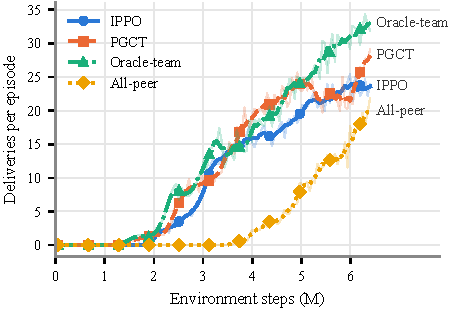
\includegraphics[width=\columnwidth]{figures/fig1_learning_curves.pdf}
\caption{Evaluation deliveries per episode during training from random initialisation in E1 (one training seed).
Thin lines: raw evaluations every 51{,}200 steps; thick lines: centred 5-point moving average.}
\label{fig:curves}
\end{figure}

\begin{table}[t]
\centering
\small
\resizebox{\columnwidth}{!}{\begin{tabular}{lcccccc}
\toprule
Method & \multicolumn{3}{c}{Onset (M steps)} & Mean deliv. & Final deliv. & Agents \\
\cmidrule(lr){2-4}
 & $\geq$1 & $\geq$10 & $\geq$20 & 0--6.4M & (last 5 evals) & learned \\
\midrule
IPPO & 2.05 & 3.17 & 5.07 & 10.4 & 23.2 $\pm$ 1.1 & 2/4 \\
PGCT & 1.79 & 3.28 & 4.15 & 11.7 & 27.3 $\pm$ 1.4 & 3/4 \\
Oracle-team & 1.64 & 2.97 & 4.66 & 13.2 & 32.2 $\pm$ 1.7 & 3/4 \\
All-peer & 3.99 & 5.32 & -- & 3.7 & 19.4 $\pm$ 1.6 & 4/4 \\
\bottomrule
\end{tabular}
}
\caption{Pilot results\pilot{} on E1 (one seed, common horizon 6.4M). Onset: first step at which the 3-point
moving average of deliveries per episode reaches the level. Final: mean $\pm$ s.d.\ of the last five evaluations.
Agents learned: agents with $\geq$1 delivery per episode over the last five evaluations.}
\label{tab:performance}
\end{table}

\textbf{Learning curves.} Oracle-team sharing produced the earliest onset and the highest curve
(Figure~\ref{fig:curves}, Table~\ref{tab:performance}): one delivery per episode was reached at 1.64M steps
vs.\ 2.05M for IPPO, with a mean
13.2 vs.\ 10.4 deliveries per episode over training and 32.2 vs.\ 23.2 at the end. PGCT lay in between.
All-peer sharing delayed learning by about two million steps but improved fastest at the end.\pilot

\begin{figure*}[t]
\centering
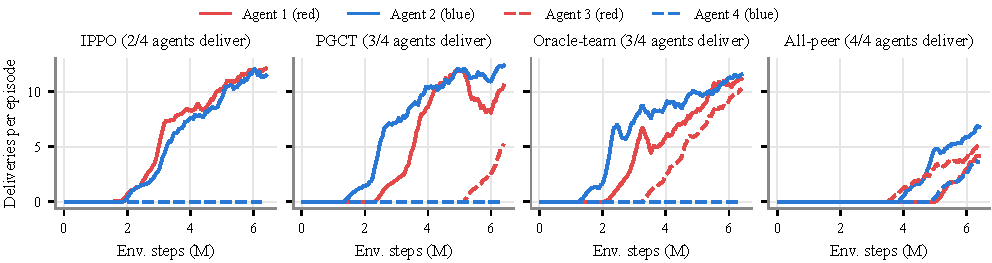
\includegraphics[width=\textwidth]{figures/fig2_per_agent_deliveries.pdf}
\caption{Deliveries per episode of each agent (5-point moving average). Red: team red (agents 1, 3); blue: team
blue (agents 2, 4); solid: agents 1--2; dashed: agents 3--4. Panel titles give the number of agents that deliver.}
\label{fig:agents}
\end{figure*}

\textbf{Sharing determines how many agents learn.} Most of the throughput difference is explained by the number
of agents that learned to deliver at all (Figure~\ref{fig:agents}): two under IPPO (one per team), three under PGCT
and Oracle-team, four under All-peer. Each agent that learned contributed about 10--12 deliveries per episode;
agents that did not learn kept moving but never picked up a requested shelf in evaluation. A plausible mechanism is
that, with individual rewards and only two requests per team, the first teammate to learn serves most requests and
the other receives too little reward to learn; distilling a competent peer's critic gives it a learning signal
without its own rewards. Under Oracle-team, the lagging teammate of agent 1 started delivering at 3.6M steps, while
the corresponding agent never did under IPPO. Sharing is not sufficient, however: agent 4 never learned under
Oracle-team although it regularly distilled from agent 2.\pilot{} This mechanism is a hypothesis; testing it requires
seeds and interventions (e.g.\ cutting distillation for the lagging agent).

\begin{figure*}[t]
\centering
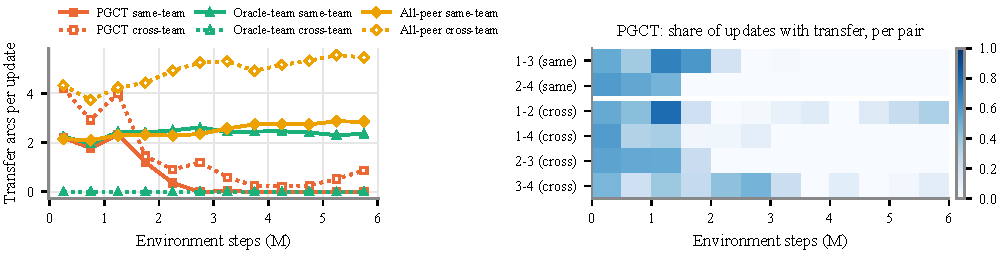
\includegraphics[width=\textwidth]{figures/fig3_critic_transfer.pdf}
\caption{Realised critic transfer (logged donor allocation, after warm-up). Left: directed transfer arcs per update,
same-team (solid) vs.\ cross-team (dotted), in 0.5M-step bins. Right: for PGCT, share of updates in which each pair
exchanged critic information.}
\label{fig:transfer}
\end{figure*}

\begin{table}[t]
\centering
\small
\resizebox{\columnwidth}{!}{\begin{tabular}{llccc}
\toprule
Method & Window & Updates w/ transfer & Same-team arcs/upd. & Cross-team arcs/upd. \\
\midrule
PGCT & 0--2.0M & 91\% & 1.86 & 3.09 \\
 & 2--4.0M & 37\% & 0.10 & 0.73 \\
 & 4--6.4M & 29\% & 0.03 & 0.63 \\
\addlinespace
Oracle-team & 0--2.0M & 82\% & 2.26 & 0.00 \\
 & 2--4.0M & 86\% & 2.50 & 0.00 \\
 & 4--6.4M & 85\% & 2.39 & 0.00 \\
\addlinespace
All-peer & 0--2.0M & 99\% & 2.22 & 4.18 \\
 & 2--4.0M & 100\% & 2.49 & 5.10 \\
 & 4--6.4M & 100\% & 2.79 & 5.37 \\
\bottomrule
\end{tabular}
}
\caption{Realised transfer per training window (one seed\pilot). Arcs are directed receiver--donor links.}
\label{tab:transfer}
\end{table}

\textbf{What the gate selects (RQ3).} During the first 2M steps the PGCT gate admitted transfer on 91\% of
updates, with more cross-team (3.09 arcs per update) than same-team (1.86) transfer, as all policies are still
similar (Figure~\ref{fig:transfer}, Table~\ref{tab:transfer}). From 2M steps on, same-team transfer almost vanished
(0.10 and 0.03 arcs per update in 2--4M and 4--6.4M) and the remaining links were cross-team, first between agents
3 and 4, later between agents 1 and 2---the two agents that delivered most. The probe-JS between teammates was
larger than between non-teammates at almost every checkpoint after 2.5M steps, for all four methods
(Figure~\ref{fig:jsgap}); sharing critics within the true team did not make teammates' actors more similar.

\begin{figure}[t]
\centering
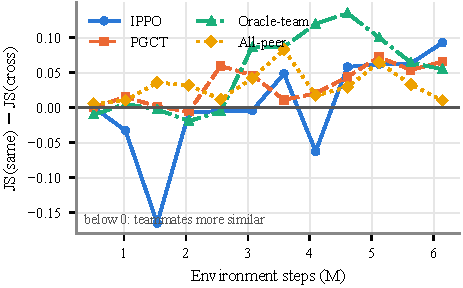
\includegraphics[width=\columnwidth]{figures/fig4_probe_js_gap.pdf}
\caption{Probe-JS between teammates minus probe-JS between non-teammates on the 48 canonical probes, computed from
checkpoints. Above zero: teammates' policies are less similar than non-teammates'.}
\label{fig:jsgap}
\end{figure}

\textbf{Roles, not teams.} A frozen analysis of an earlier curriculum model (trained with 50\% of shelves in the
other team's half) shows the structure that the gate picks up (Appendix~\ref{app:roles}). Agents 1 and 2 worked
almost exclusively in their own team's half of the map (99.6\% and 99.5\% of steps), whereas agents 3 and 4
fetched most of their team's requested shelves from the other half and spent about 76\% of their time carrying.
The two ``long-haul'' agents belong to different teams but behave alike, and they were the pair the gate linked
most (1{,}170 updates). In the same curriculum, the same-team gate distances were 0.086 and 0.100 when each team's
shelves were confined to its own half and rose to 0.26 and 0.32 as soon as 12.5\% of the shelves were mixed.
Behavioural similarity therefore tracks role and skill; in E1 these are not aligned with team membership.

\textbf{Reproducibility.} Re-running the same seed with identical initial weights reproduced IPPO exactly
(evaluation curves identical up to 2.46M steps), but the three sharing variants diverged from the earlier run after
1.38--1.59M steps (Appendix~\ref{app:repro}), presumably because of non-deterministic GPU operations in the
distillation path (not yet verified). The divergence was large: the delivery onset of All-peer moved from
1.89M to 3.99M steps. Comparisons between sharing methods therefore require several independent seeds.

\section{Discussion}
\textbf{What the evidence supports.} (i) In a team-symmetric task, probe-based policy similarity does not identify
teams and is dominated by role and skill; this holds across frozen checkpoints, probe designs and a from-scratch run.
(ii) Information that does identify teams---locally witnessed task events---is available to the agents
under the stated observation assumptions. (iii) In one seed, sharing critics with the true team gave the best
learning curve, and broader sharing let more agents learn; both need replication.

\textbf{What it does not support.} We do not claim that PGCT or any inferred-team method improves learning, that
oracle sharing reliably helps, or that the observed mechanism (rescuing lagging agents) is causal. Probe-JS failing
in E1 is expected from the symmetry of the task and may change when teams' objectives differ.

\textbf{Assumptions.} Local task evidence requires that an observer can attribute an observed event to a specific
neighbour (the observation grid contains no agent identifiers) and that it knows its own objective. If agents
could simply communicate their team identifiers, team inference would be unnecessary; the setting is relevant
when objectives are private, labels are not shared across organisations, or groups emerge without a common
vocabulary. These assumptions must be made explicit in any claim of decentralised team discovery.

\textbf{Next steps.} \todo{Fill in after the runs finish.} (1) Seeds 2--3 (or more) of the E1 comparison, with
the number of agents that learn as an explicit metric. (2) E1-F, where team goals are at opposite corners: does team
behaviour diverge, does the ``carrying, no goal visible'' probe bank separate teams, and does Oracle-team sharing
gain over All-peer when teams' value functions differ? (3) An online gate driven by local task evidence instead of
probe similarity, compared against Oracle-team, All-peer and IPPO; (4) MAPPO and SePS-style baselines once a
condition with a reliable effect is established.

\section{Conclusion}
Behavioural similarity is an appealing, decentralised proxy for whom to share with, but in our warehouse study it
measured role and skill rather than team membership: a similarity-gated critic sharing method gradually linked
agents across teams, while locally witnessed task outcomes identified teams immediately. Sharing with the right
partners looked beneficial in a pilot, mainly by helping lagging agents learn. Establishing that inferred teams
improve learning requires separating identifiability, the value of oracle sharing and the behaviour of the inferred
gate---and multiple seeds, because sharing methods amplify small numerical differences.

\ifdefined\ijcaistyle
  \bibliographystyle{named}
\else
  \bibliographystyle{plainnat}
\fi
\bibliography{references}

\clearpage
\appendix
\onecolumn

\section{Hyper-parameters}
\label{app:hyper}
\begin{table}[h]
\centering
\small
\begin{tabular}{ll}
\toprule
Setting & Value \\
\midrule
Map / agents / teams & 11$\times$10 E1 / 4 / 2 \\
Reward & individual \\
Home-zone shelf ratio & 0.5 \\
Requests per team & 2 \\
Sensor / communication range & 5 / 5 \\
Learning rate & 0.0002 \\
Entropy coef. & 0.05 \\
$\gamma$ / GAE $\lambda$ & 0.99 / 0.95 \\
Rollout / BPTT length & 1024 / 64 \\
PPO epochs / minibatches / clip & 4 / 8 / 0.2 \\
Hidden (MLP / GRU) & 128 / 128 \\
Peer-loss coef. $\lambda_{peer}$ & 0.01 \\
Gate: JS threshold / EMA $\beta$ / warm-up & 0.12 / 0.35 / 100 upd. \\
Canonical probes & 48 (fixed, zero hidden, length 1) \\
Evaluation & every 50 updates, 20$\times$500 steps, deterministic \\
\bottomrule
\end{tabular}

\caption{Settings of the from-scratch E1 comparison (identical for all methods except the distillation gate).}
\end{table}

\section{Probe banks on frozen E1 models}
\label{app:frozen}
\begin{figure}[h]
\centering
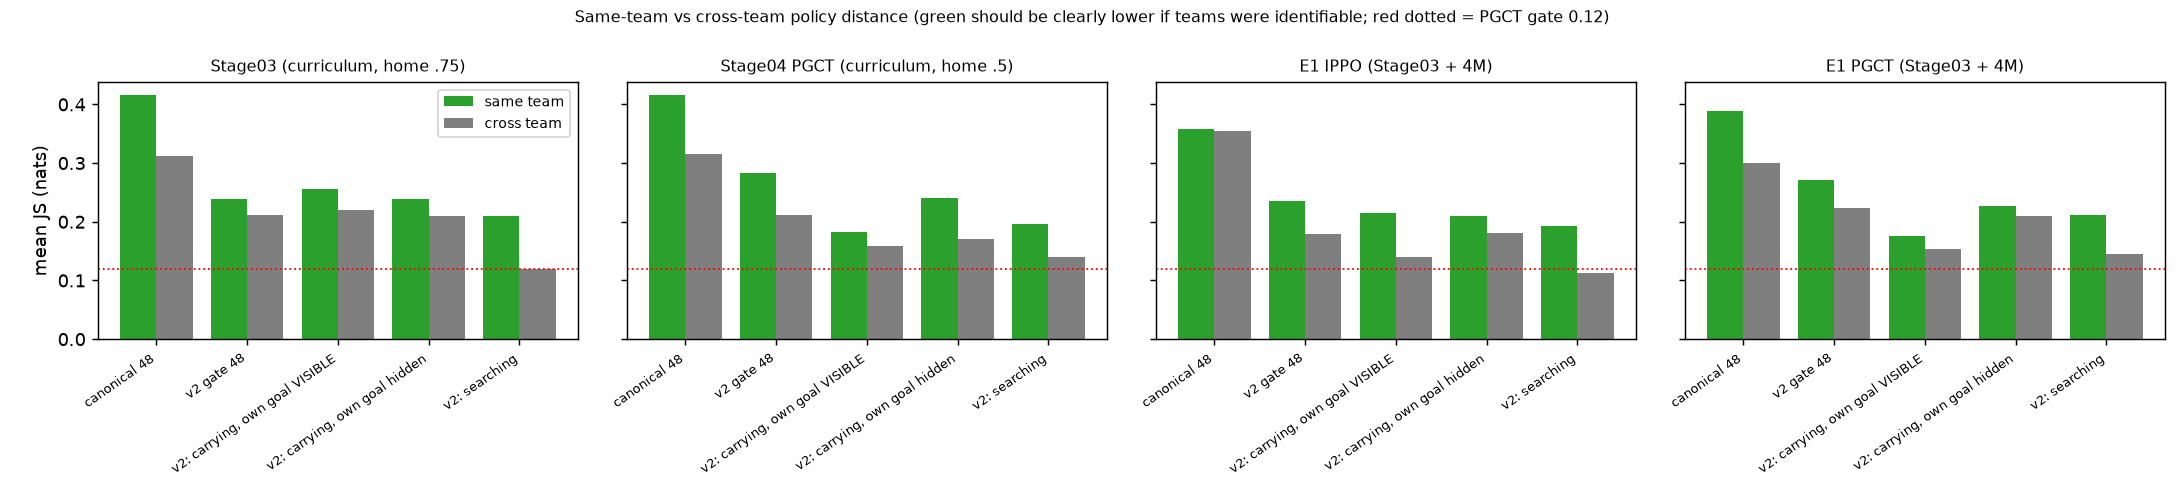
\includegraphics[width=\textwidth]{figures/frozen_probe_same_vs_cross.png}
\caption{Mean probe-JS between teammates (green) and non-teammates (grey) for four frozen E1 models and five probe
subsets: the canonical bank, the ``carrying, no goal visible'' bank, and transfer-bank subsets (carrying with own goal
visible, carrying with goal hidden, searching). Teammates are less similar in all 20 combinations. Red dotted line:
gate threshold 0.12.}
\end{figure}

\section{Spatial roles in a curriculum model}
\label{app:roles}
\begin{figure}[h]
\centering
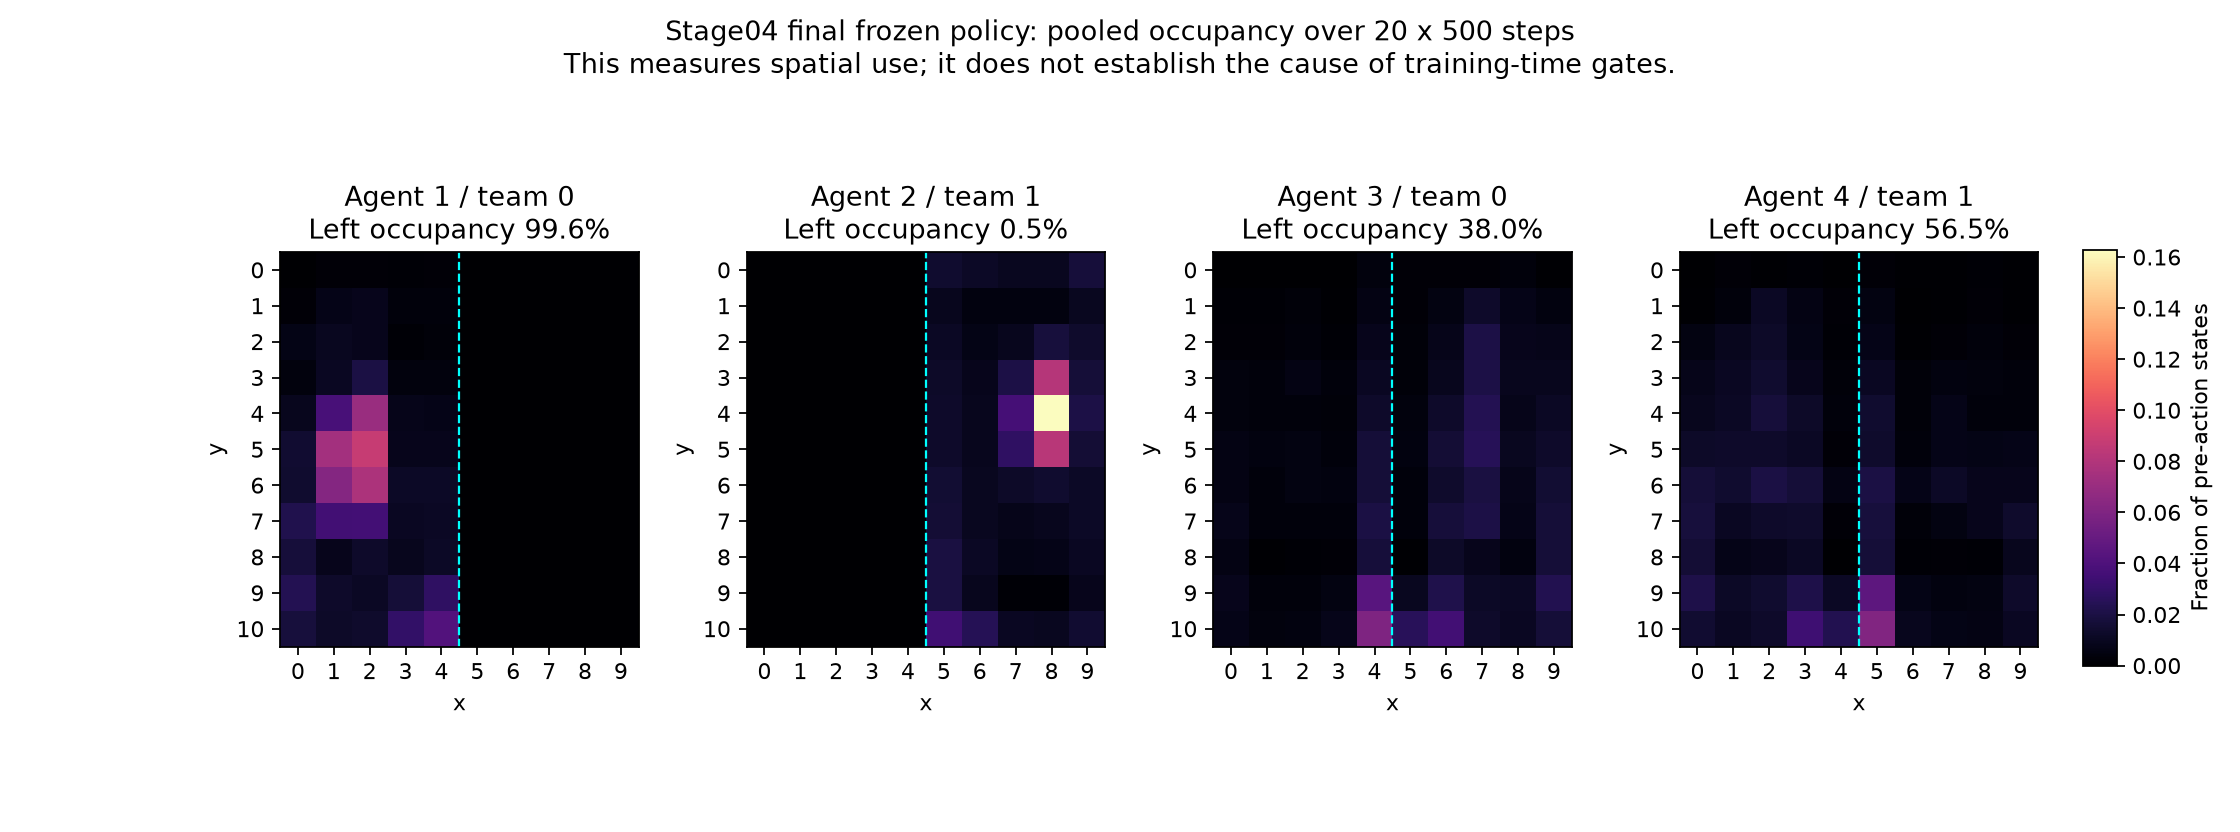
\includegraphics[width=\textwidth]{figures/stage04_occupancy.png}
\caption{Cell occupancy of a frozen curriculum model (Stage04, 50\% of shelves in the other team's half) over
20$\times$500 steps. Agents 1 and 2 stay in their own team's half; agents 3 and 4 fetch shelves from the other half.}
\end{figure}

\section{Probe-JS at selected checkpoints}
\begin{table}[h]
\centering
\small
\begin{tabular}{lcccc}
\toprule
Method & \multicolumn{4}{c}{JS same-team / cross-team at} \\
\cmidrule(lr){2-5}
 & 1M & 2M & 4M & 6M \\
\midrule
IPPO & 0.03 / 0.07 & 0.16 / 0.17 & 0.17 / 0.23 & 0.27 / 0.18 \\
PGCT & 0.07 / 0.06 & 0.16 / 0.16 & 0.17 / 0.15 & 0.26 / 0.19 \\
Oracle-team & 0.07 / 0.06 & 0.16 / 0.18 & 0.31 / 0.19 & 0.29 / 0.23 \\
All-peer & 0.09 / 0.08 & 0.22 / 0.19 & 0.23 / 0.21 & 0.15 / 0.14 \\
\bottomrule
\end{tabular}

\caption{Mean canonical probe-JS between teammates / between non-teammates in the from-scratch run (one seed).}
\end{table}

\section{Reproducibility with an identical seed}
\label{app:repro}
\begin{figure}[h]
\centering
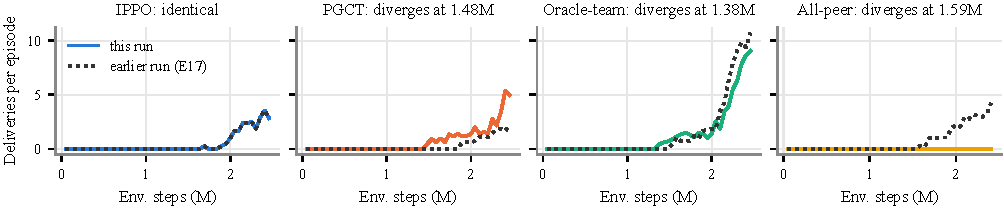
\includegraphics[width=\textwidth]{figures/figA1_reproducibility.pdf}
\caption{Two runs with the same seed and initial weights (solid: this run; dotted: an earlier interrupted run).
IPPO is reproduced exactly; the sharing variants diverge after 1.4--1.6M steps.}
\end{figure}

\section{Continuation from a shared pretrained model}
Before the from-scratch study, PGCT and IPPO were continued for 4M steps from a common curriculum checkpoint
(one seed). Normalised delivery AUC was 45.86 vs.\ 44.57 on E1 and 34.17 vs.\ 34.24 on E2; final critic
accuracy on Monte-Carlo returns was not better with PGCT. On E1 the gate never opened between teammates during this
phase (0 of 4{,}435 same-team candidate updates) and opened for the cross-team pair 3--4 on 2{,}005 of 2{,}525
candidates. These conditional results motivated the from-scratch comparison.

\end{document}
